%!TEX root = ../Thesis.tex

\chapter{Clusteranalyse von Fahrzeugtrajektorien}
\label{cha:realisation_clustering}

In diesem Kapitel wird die Umsetzung der Clusteranalyse der Trajektorien vorgestellt.
Es wird zuerst darauf eingegangen, welche Trajektorie-Repräsentation gewählt wurde. Anschließend
werden die verschiedenen Schritte zur Bereinigung und Vorverarbeitung der Daten beschrieben, welche
in dieser Arbeit zum Einsatz kommen. Schlussendlich folgt die Erläuterung der eigentlichen Clusteranalyse.
Hier werden die verschiedenen untersuchten Ansätze vorgestellt und ihre Ergebnisse diskutiert.

Die \textit{TrackerApplication} ist in Java und Scala implementiert. Ihre Benutzeroberfläche basiert
auf JavaFX. Das in dieser Arbeit erstellte Modul \textit{Spurerkennung} wird komplett mit Scala umgesetzt.

\section{Trajektorie-Definition}

Die Ergebnisse der Fahrzeugverfolgung (siehe Abschnitt \ref{sec:position_extraction}) werden
in der \textit{TrackingApplication} in Form sogenannter \textit{TrackedObject}`s gespeichert.
Ein solches Objekt repräsentiert eine zusammenhängende, nicht unterbrochene Verfolgung eines Fahrzeugs.
Wird eine Verfolgung, beispielsweise aufgrund einer Überdeckungen, unterbrochen, so existieren für ein
Kraftfahrzeug mehrere Objekte, welche sich einander nicht zuordnen lassen.
Die wichtigsten Informationen, die ein \textit{TrackedObject} beinhaltet, sind eine eindeutige ID,
die Frame-Positionen des Starts und Endes der Verfolgung und die Objekt-Klasse des Fahrzeugs. Es wird
zwischen den vier Klassen \textit{``Auto''}, \textit{``Lastwagen''}, \textit{``Transporter''}
und \textit{``Zweirad''} unterschieden.
Für jedes verfolgte Objekt können die zugehörigen Positions-, Geschwindigkeits-, Beschleunigungs-
und Dimensions-Informationen abgerufen werden. Diese werden für jedes Frame, welches zwischen dem Start-
und End-Frame des Objektes liegt, bestimmt.

Da für die Ableitung von Fahrspuren aus Trajektorien lediglich die positionsbezogenen Eigenschaften
der Fahrzeuge relevant sind, werden Bewegungbahnen in dieser Arbeit über jene definiert.
Geschwindigkeit, Beschleunigung und Dimension der Fahrzeuge wird in der Clusteranalyse nicht berücksichtigt.
Abbildung \ref{fig:real_trajectory_classDia} zeigt den Aufbau einer Trajektorie im Modul \textit{Spurerkennung}.

\begin{figure}[H]
\centering
    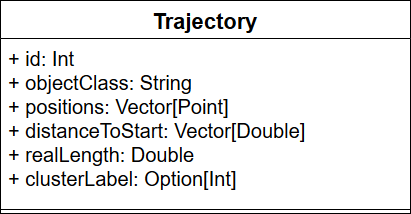
\includegraphics[width=0.38\linewidth]{../resources/img/umsetzung/U1/Trajectory_ClassDia}
\caption{Aufbau Trajektorie-Klasse}
\label{fig:real_trajectory_classDia}
\end{figure}

Die Felder \textit{id} und \textit{objectClass} werden aus dem der Trajektorie zugrundeliegenden \textit{TrackedObject}
übernommen.
Die Positionen eines Fahrzeugs werden in Form von 2D-Welt-Koordinaten (siehe Abschnitt \ref{sec:position_extraction})
in \textit{positions} gespeichert und die Anzahl der Koordinaten zusätzlich in \textit{pointLength}.
Die Sequenz \textit{distToStart} enthält für jeden Punkt der Bewegungsbahn die Distanz zum Start der Trajektorie in Metern.
Die Werte ergeben sich aus Formel \ref{eq_real_distToStart}, wobei $p_n$ dem $n$-ten Punkt in der Trajektorie entspricht
und $dist$ der euklidschen Distanz zwischen zwei Punkten.

\begin{ceqn}
\begin{align}
\label{eq_real_distToStart}
    distToStart(p_n) =
    \begin{cases}
        0 & \text{if } n = 0 \\
        dist(p_n,\ p_{n-1}) + distToStart(p_{n-1}) & \text{otherwise}
    \end{cases}
\end{align}
\end{ceqn}

Aus \textit{distToStart} ergibt sich zudem die Gesamtlänge einer Trajektorie, welche extra gespeichert wird.
Das Feld \textit{clusterLabel} ordnet jede Trajektorie nach der Clusteranalyse einem bestimmten Cluster zu.
Zuvor enthält es keinen Wert.

% TODO: Evtl Bilder und Beschreibung austauschen
Zur Untersuchung der Fahrzeugtrajektorien ist es hilfreich diese zu visualisieren. Abbildung \ref{fig:real_trajs_raw_neckartor}
zeigt so beispielsweise 1240 Trajektorien, welche aus einer Aufnahme des Stuttgarter Neckartors extrahiert wurden.
In Abbildung \ref{fig:real_neckartor} ist ein Ausschnitt der entsprechenden Aufnahme zu sehen.

\begin{figure}[H]
\centering
    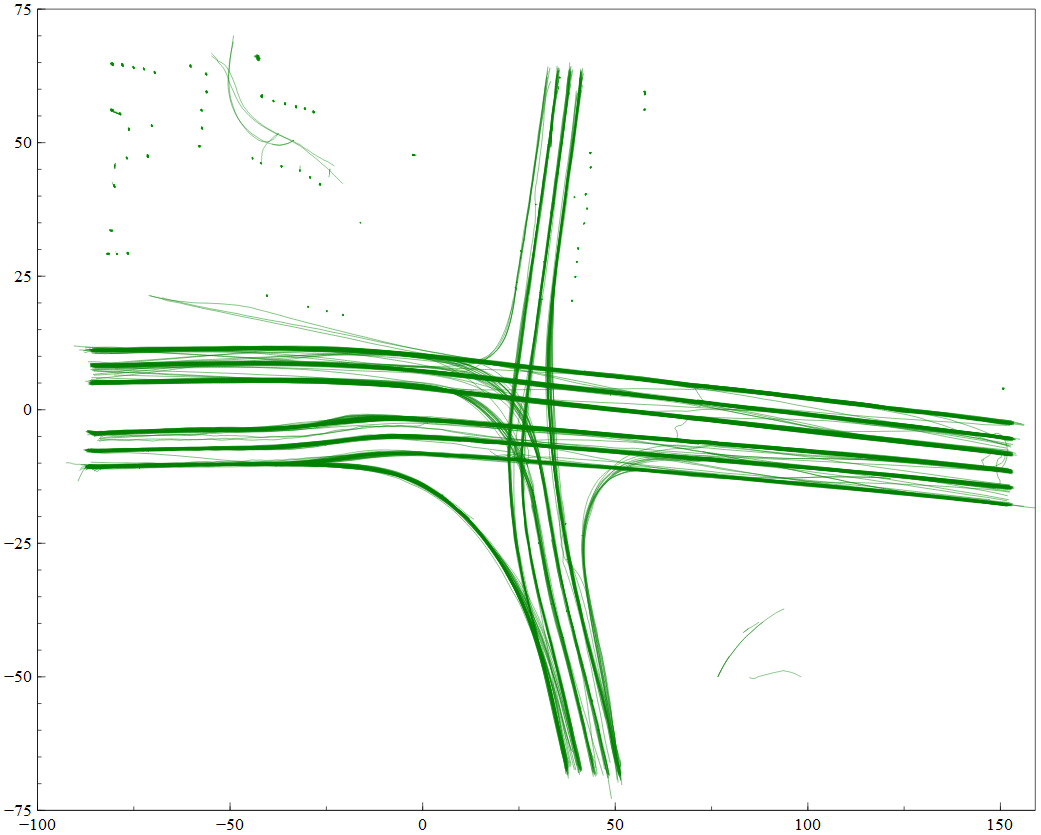
\includegraphics[width=0.5\linewidth]{../resources/img/umsetzung/U1/Plot_RawTrajectories_Neckartor}
\caption{Unverarbeitete Trajektorien vom Stuttgarter Neckartor}
\label{fig:real_trajs_raw_neckartor}
\end{figure}

\begin{figure}[H]
\centering
    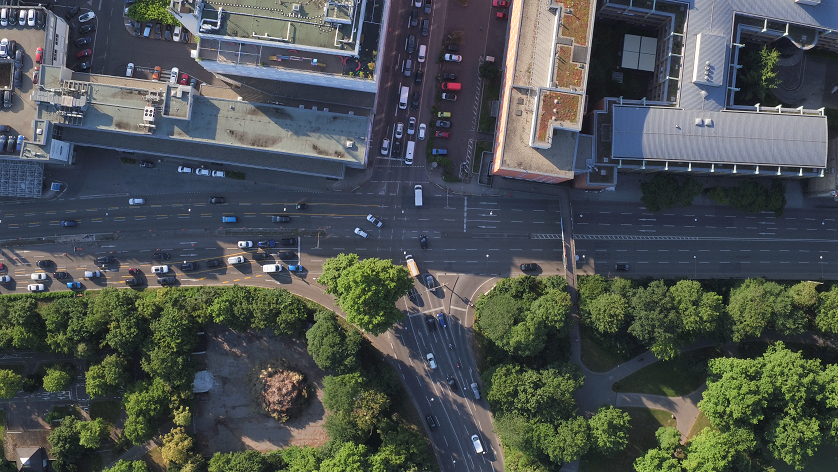
\includegraphics[width=0.7\linewidth]{../resources/img/umsetzung/U1/Neckartor_Aufnahme}
\caption{Das Stuttgarter Neckartor}
\label{fig:real_neckartor}
\end{figure}

In Abbildung \ref{fig:real_trajs_raw_neckartor} sind die verschiedenen Bewegungsbahnen der Fahrzeuge für
den menschlichen Betrachter bereits klar erkennbar.
Direkt fallen aber auch die Trajektorien der stehenden oder sich auf Parkplätzen
bewegenden Autos im oberen Bereich der Aufnahme ins Auge. Diese dürfen nicht in die Clusteranalyse mit einbezogen werden.
Bei genauerer Untersuchung der Trajektorien zeigen sich weitere Probleme, welche das Clustering negativ
beeinflussen würden. Zwei sind in nachfolgender Abbildung dargestellt.
\ref{fig:real_defects_trajectories} a) zeigt, wie Fahrzeuge Punktwolken beim Stilstand vor Lichtsignalanlagen bilden.
In \ref{fig:real_defects_trajectories} b) wird deutlich, dass in manchen Bereichen sehr viele Trajektorie-Unterbrechungen
auftreten. Hier wird die Straße üblicherweise von Bäumen, Brücken et cetera überlagert.

\begin{figure}[H]
    \centering
    \subfloat[]{{
        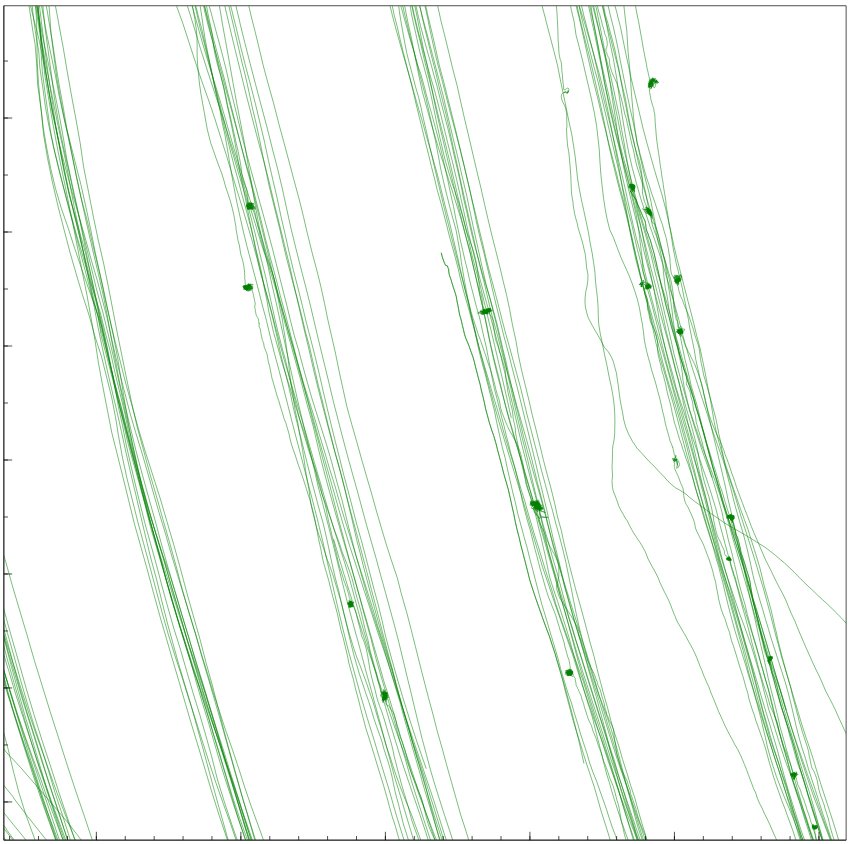
\includegraphics[align=c, width=0.35\linewidth]{../resources/img/umsetzung/U1/trajectories_defect1}
    }}
    \qquad
    \subfloat[]{{
        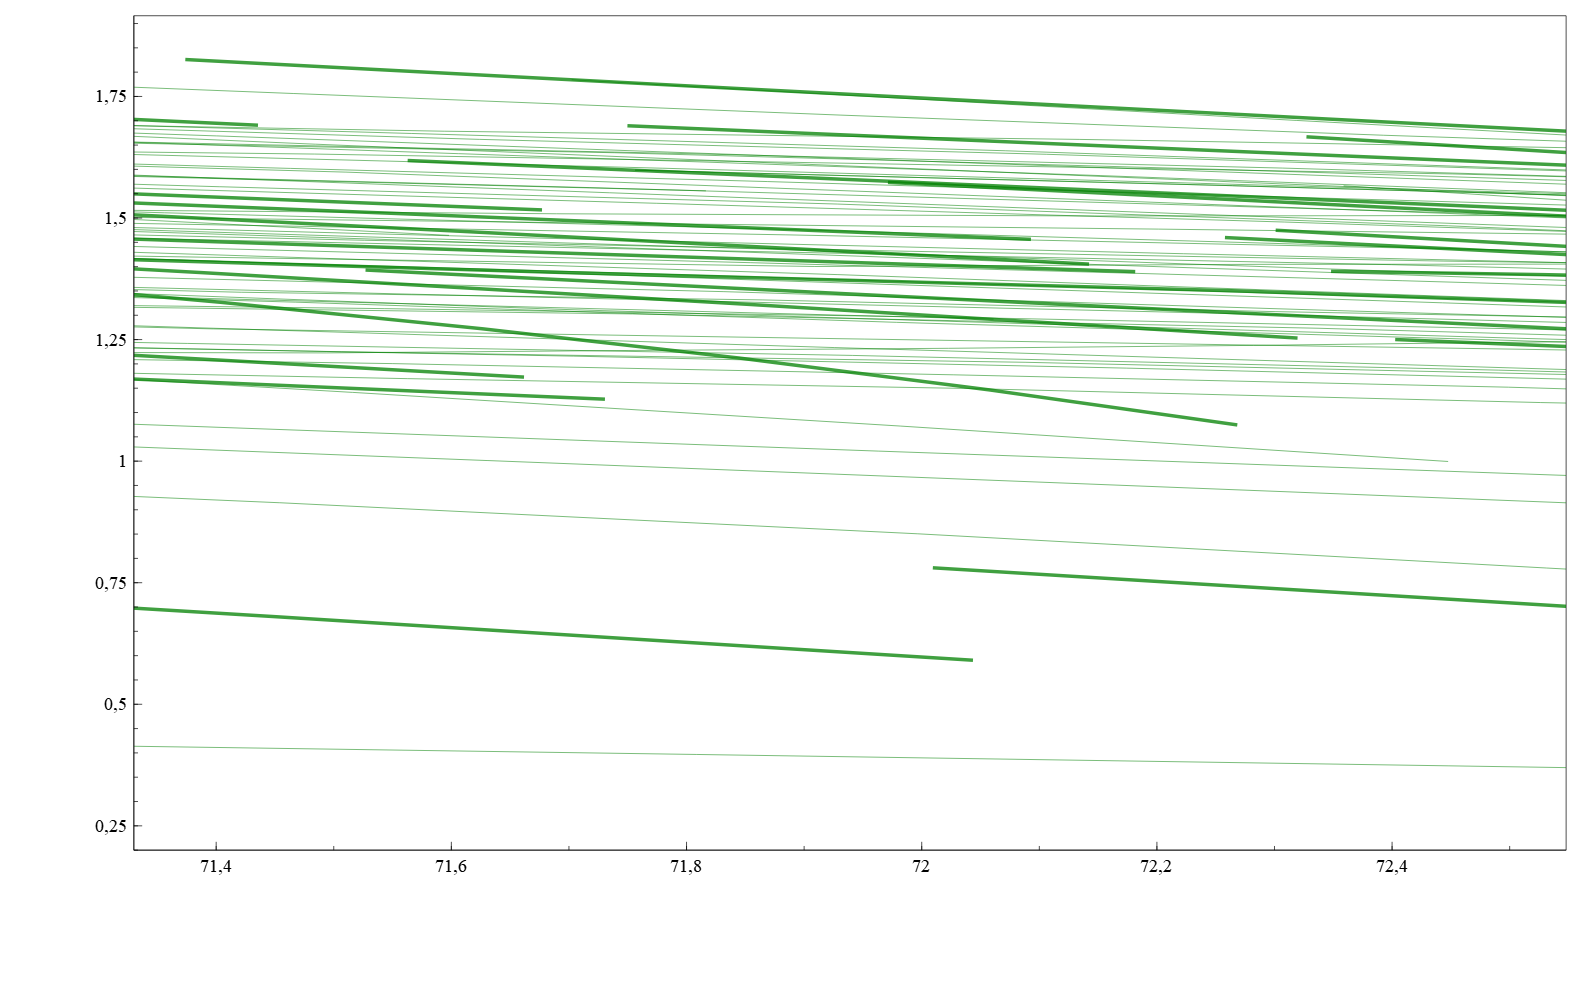
\includegraphics[align=c, width=0.45\linewidth]{../resources/img/umsetzung/U1/trajectories_defect2}
    }}
    \caption{a) Punktwolken vor Lichtsignalanlagen, b) Unterbrechungen aufgrund von Überdeckung}
    \label{fig:real_defects_trajectories}
\end{figure}

Um von diesen und weiteren Effekten bei der Clusteranalyse nicht beeinflusst zu werden, durchlaufen die
``Roh-Trajektorien'' einen Vorverarbeitungsschritt. Dieser wird im nächsten Abschnitt vorgestellt.

\section{Vorverarbeitung der Trajektorien}
\label{sec:realisation_preprocessing}

Die verschiedenen Schritte, welche zur Vorverarbeitung und Bereinigung der Roh-Trajektorien angewandt werden,
sind in diesem Abschnitt geschildert.

Das primäre Ziel der Vorverarbeitung ist es, Ausreißer aus der
Trajektorie-Menge zu entfernen, welche das Ergebnis der Clusteranalyse negativ beeinflussen könnten.
Idealerweise sollen nur jene Trajektorien beibehalten werden, welche eine komplette Bewegung eines
Fahrzeugs auf einem bestimmten Straßenabschnitt repräsentieren. Anhand dieser Trajektorien kann
anschließend die Geometrie der realen Fahrspuren ermittelt werden. Ausreißer wie stehende oder unterbrochene Trajektorien
liefern hingegen keine verwendbaren Informationen für die Spurerkennung.

In nachfolgender Auflistung sind die vier wichtigsten Vorverarbeitungsschritte und ihre Anwendungsreihenfolge
aufgeführt. Die einzelnen Schritte und ihr Hintergrund werden anschließend noch genauer erläutert.

\begin{enumerate}
    \item Resampling von Trajektorien auf minimale Punktdistanz
    \item Entfernung zu kurzer Trajektorien
    \item Entfernung unterbrochener Trajektorien
    \item Anpassung der Trajektorien bei niedrigen Aufnahmewinkeln
\end{enumerate}

\subsection{Resampling von Trajektorien auf minimale Punktdistanz}
Der erste Vorverarbeitungsschritt reduziert die Anzahl der Koordinaten, welche eine Bewegungsbahn beschreiben, erheblich
ohne dabei jedoch wichtige Informationen zu verlieren. Insbesondere dann, wenn sich Fahrzeuge mit niedrigen
Geschwindigkeiten bewegen oder teilweise von Ampeln et cetera. stehen, bestehen die Roh-Trajektorien aus sehr vielen
Punkten, welche oft beinahe identische Positionsinformationen darstellen, das heist nur sehr geringe
Abstände voneinander haben. Für die Beschreibung einer Bewegungsbahn ist diese Punktdichte nicht notwendig
und sogar kontraproduktiv, da sie die Performance der nachfolgenden Schritte stark erhöht. Hiervon ist insbesonders
die Clusteranalyse betroffen.

Aus diesen Gründen werden im ersten Vorverarbeitungsschritt Trajektorien auf eine minimale Punktdistanz
von $0.5\ m$ gebracht. Der hierzu verwendete Algorithmus ist in Listing \ref{lst:pseudo_resampling} dargestellt.
Er verwirft alle aufeinanderfolgende Punkte, welche von einem Referenzpunkt weniger als den geforderten Abstand haben.

\begin{lstlisting}[caption=Pseudocode Trajektorie Resampling, language=FSharp, label=lst:pseudo_resampling]
algorithm resampleTrajectory:
  input:  lastRefPoint
          newTrajPoints
          oldTrajPoints
  output: resampled trajectory points

  while oldTrajPoints is not empty do:
    nextPoint := Head(oldTrajPoints)
    remPoints := Tail(oldTrajPoints)

    if dist(lastRefPoint, nextPoint) < 0.5:
      resampleTrajectory(lastRefPoint, newTrajPoints, remPoints)
    else:
      resampleTrajectory(nextPoint, newTrajPoint ++ nextPoint, remPoints)

  return newTrajPoints
\end{lstlisting}

Nach Anwendung des Algorithmus ist im Fall der Neckartor Aufnahme die durchschnittliche Punktlänge
der Trajektorien von 1094 Koordinaten auf 160 gesunken. Die realen Längen der Bewegungsbahnen bleiben
hingegen nahezu gleich. Die Punktwolken, welche stehende Fahrzeuge erzeugen, werden mittels dieses
Schritts ebenfalls entfernt (siehe Abb. \ref{fig:real_result_2nd_Prepro} b)).


\subsection{Entfernung zu kurzer Trajektorien}
Der zweite Verarbeitungsschritt ist sehr einfach aber dennoch sehr effektiv, da mit seiner Hilfe viele
Trajektorien von beispielsweise stehenden Fahrzeugen oder kurz auftretende Tracking-Fehler entfernt
werden können. Hierzu werden die Längen aller Trajektorien überprüft und jene entfernt, welche
unter bestimmten Grenzwerten liegen. Die hierzu verwendete boolesche Überprüfung ist in Gleichung
\ref{eq_isShortTrajectory} gegeben. Die Grenzwerte würden experimentell bestimmt und lieferten für die
Testaufnahmen gute Ergebnisse.

\begin{ceqn}
\begin{align}
\label{eq_isShortTrajectory}
    isShortTrajectory(t) =
    \begin{cases}
        1 & \text{if } t.pointLength < 50 \lor t.realLength < 10.0 \\
        0 & \text{otherwise}
    \end{cases}
\end{align}
\end{ceqn}

Das Ergebnis der ersten beiden Vorverarbeitungsschritte ist in Abbildung \ref{fig:real_result_2nd_Prepro} dargestellt.
Die Trajektorien stehender Fahrzeuge, sowie die Punktwolken vor Lichtsignalanlagen und weitere Defekte aufgrund
kleiner Tracking-Fehler wurden entfernt.

\begin{figure}[H]
    \centering
    \subfloat[]{{
        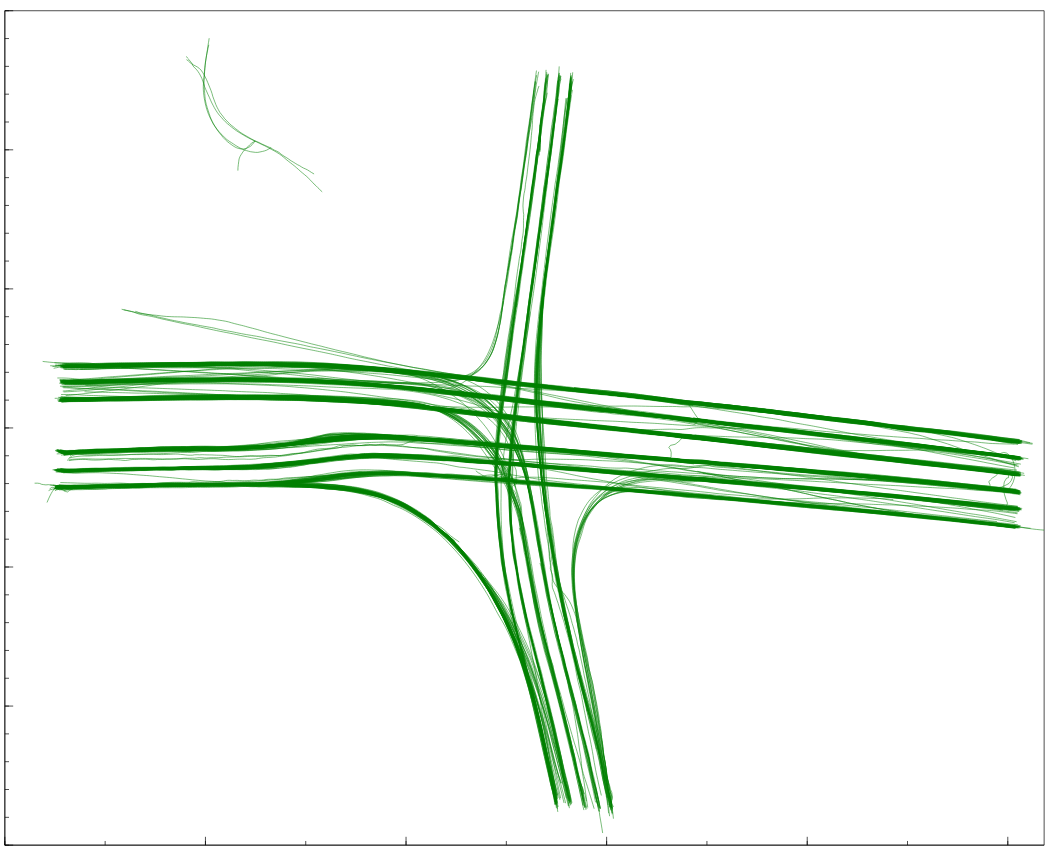
\includegraphics[align=c, width=0.41\linewidth]{../resources/img/umsetzung/U1/trajectories_resampledFiltered}
    }}
    \qquad
    \subfloat[]{{
        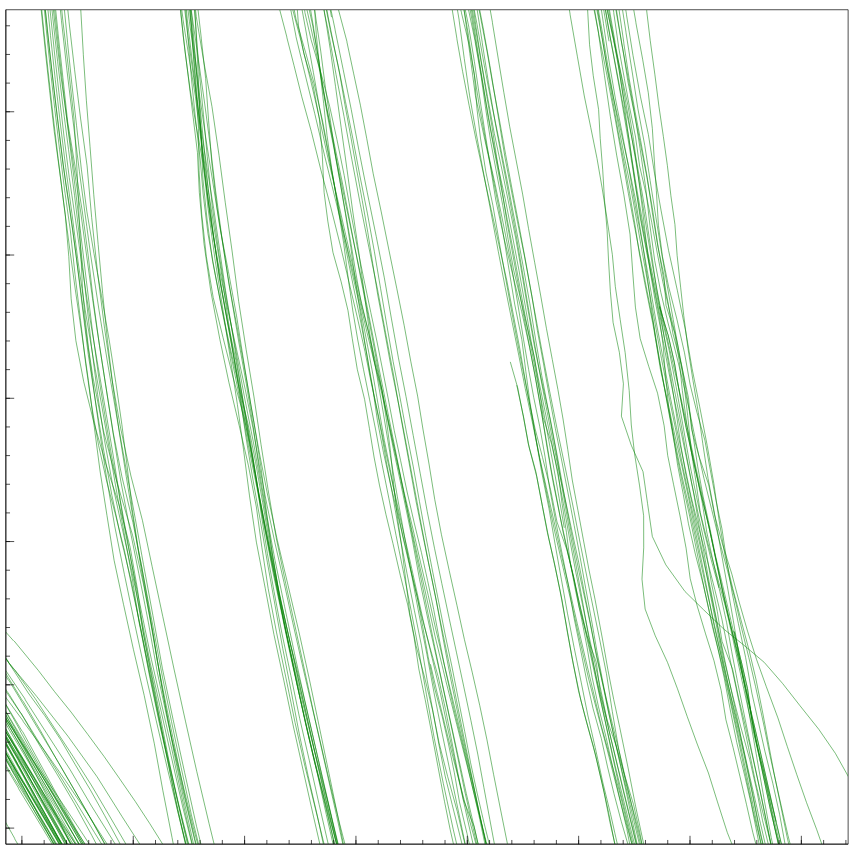
\includegraphics[align=c, width=0.34\linewidth]{../resources/img/umsetzung/U1/trajectories_resampled_cleared}
    }}
    \caption{Ergebnisse der zwei ersten Vorverarbeitungsschritte}
    \label{fig:real_result_2nd_Prepro}
\end{figure}

\subsection{Entfernung unterbrochener Trajektorien}

Nachdem die ersten beiden Verarbeitungsschritte bereits stehende Trajektorien entfernt haben,
müssen nun noch unterbrochene Verfolgungen ausgefiltert werden. Hierzu wird angenommen, dass komplette
Bewegungsbahnen immer im Bereich der Szenenränder beginnen und enden. Wurde eine Fahrzeugverfolgung
unterbrochen, so befinden sich die Anfänge beziehungsweise Enden der daraus resultierenden Trajektorien
im Innenbereich der Aufnahme. Diese Trajektorien werden entfernt. Abbildung \ref{fig:real_completeTrajectory_Definition}
veranschaulicht das Prinzip der Szenen Rand- und Innenbereiche.

\begin{figure}[H]
\centering
    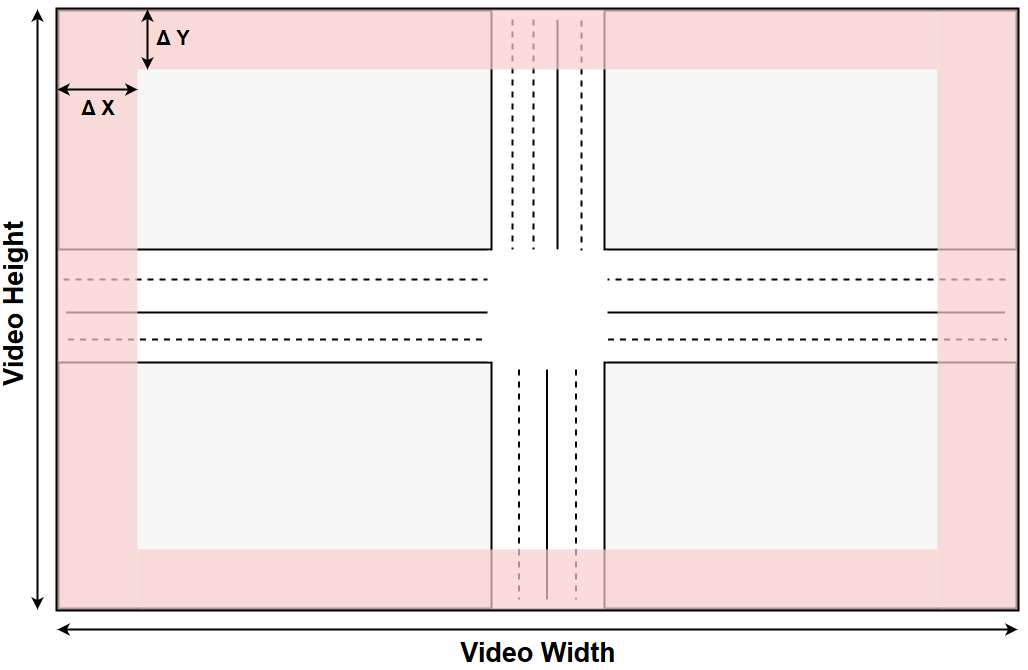
\includegraphics[width=0.5\linewidth]{../resources/img/umsetzung/U1/LaneTopo_CompleteTra}
\caption{Definition von Szenen Rand- und Innenbereich}
\label{fig:real_completeTrajectory_Definition}
\end{figure}

Die Werte $\Delta X$ und $\Delta Y$ entsprechen 10\% der Video-Breite beziehungsweise Höhe.
Ob sich eine Punkt $p$ innerhalb des Szenenrandes befindet, wird mit Hilfe von Formel \ref{eq_inSceneFringe} überprüft.
Hierbei entsprechen $p.sX$ und $p.sY$ den Bildkoordinaten des Punktes $p$.

\begin{ceqn}
\begin{align}
\label{eq_inSceneFringe}
    inSceneFringe(p) =
    \begin{cases}
        1 & \text{if } (p.sX < \Delta X \lor (p.sX > (vWidth - \Delta X))) \\
          &            \lor\ ((p.sY < \Delta Y) \lor (p.sY > (vHeight - \Delta Y))) \\
        0 & \text{otherwise}
    \end{cases}
\end{align}
\end{ceqn}

Nach Ausführung dieses Filter-Schrittes, besteht die Menge der übrigen Trajektorien grundsätzlich nurnoch
aus kompletten Bewegungsbahnen.

Dieser Vorverarbeitungsschritt beruht auf der Annahme, dass für eine Fahrspur neben unterbrochenen auch
ununterbrochene Trajektorien vorliegen, welche eine vollständige Bewegung auf der Spur beschreiben.
Sind alle Trajektorien einer Fahrspur aufgrund einer Verdeckung in der Aufnahme unterbrochen, werden
diese durch das Verfahren vollständig entfernt und eine Extraktion der Spur ist nicht möglich.

\subsection{Anpassung der Trajektorien bei niedrigen Aufnahmewinkeln}


% Endnotes:
%   Problematisch auch Spurwechsel. Hier schwer auszufiltern, da sie Ausreißer in Bezug auf eine Spur darstellen
%   und nicht generelle Ausreißer

\section{Clusteranalyse}
\label{sec:realisation_clustering}

% genaue Beschreibung des Vorgehens, bis finale Clustering Lösung erreicht wurde
% Ansätze: Gründe, Stärken, tatsächliche Problem
% Ansatz A:
%   Mod. Hausdorff Distanz und Spectral Clustering (bas. auf Avet et al.) (Erklärung Grundfunktionsweise Spectral-Clustering)
%   Weil: SC performant, deterministisch, oft verwendet
%   Probleme: Clusteranzahl Bestimmung, Umgehen mit Ausreißern, Tatsächliche Ergebnisse nicht gut
%   --> Performance / Qualität des Ansatzes konnte für vorhandene Daten nicht bestätigt werden
%   --> Problematisch auch Umgang mit vielen Parametern

% Probleme: Erkennung von Abbiegespuren, mit wenig Fahrzeugen und Abbiegevorgängen auf mehrere Spuren
%   Dafür: Weitere Verarbeitung der Clustering Outlier
%   Beschreibung Verfahren (dichte-basiert, suchen von initial Dichten Regionen, Verfolgung bis Ausdünnung)

Nachdem im vorherigen Abschnitt beschrieben wurde, wie die Roh-Trajektorien vorverarbeitet und gefiltert
werden, folgt nun die Erläuterung der verwendeten Ansätze zur Clusteranalyse der bereinigten Trajektorien.

\subsection{Ansatz Spectral-Clustering und modifizierte Hausdorff-Distanz}

Als erster Ansatz für die Clusteranalyse wurde das von \cite[]{Atev2010} vorgestellte Verfahren untersucht.
Es wurde gewählt, da es sowohl in der Arbeit von Atev et al. selbst, sowie auch in\cite[]{Morris2009}, gute Ergebnisse
bei der Clusteranalyse brachte.
Das Verfahren beruht auf der in \cite[]{Atev2006} vorgestellten modifizierten Hausdorff Distanz und dem
Spectral-Clustering-Algorithmus. Die Grundlagen des Distanzmaßes wurden bereits in Abschnitt
\ref{sec:atev_et_al} beschrieben. Nachfolgend wird zuerst genauer beschrieben, wie die
modifizierte Hausdorff Distanz berechnet wird und in dieser Arbeit implementiert wurde. Anschließend
wird auf den eingesetzten Spectral-Cluster-Algorithmus und die erzielten Ergebnisse eingegangen.

\subsubsection{Das Verfahren}

Grundlegend war die modifizierte Hausdorff Distanz nach Atev et al., wie in Gleichung \ref{eq_modHausdorff}
bereits definiert, gegeben über:

\begin{ceqn}
\begin{align*}
    h_{\alpha, N, C}(P, Q) = \overset{\alpha}{\underset{p \in P}{ord}}\ \Big\{ \underset{q \in N_Q(C_{P,Q}(p))}{min} d(p, q) \Big\}
\end{align*}
\end{ceqn}

Um die Distanz zwischen zwei Trajektorien $P$ und $Q$ zu bestimmen, müssen zuerst die minimalen Distanzen
zwischen allen Punkten $p \in P$ und deren Nachbarschaften $N_Q(C_{P,Q}(p))$ in $Q$ bestimmt werden.
Eine Nachbarschaft in $Q$ um den Punkt $q_0$ ist in Abhängigkeit des Parameters $w$ definiert als:

\begin{ceqn}
\begin{align}
    N_Q(q_0) = \{ q \in Q |\ |\pi_Q(q_0) - \pi_Q(q)| \le w/2 \}
\end{align}
\end{ceqn}

$\pi_Q(q)$ entspricht hierbei der relativen Position von $q$ in $Q$, welche in Gleichung \ref{eq_atev_relPos} definiert ist.
$|Q_j|$ steht für die Länge einer Trajektorie bis zum Punkt $j$ und $|Q|$ für die Gesamtlänge einer Bewegungsbahn.
Diese Längeninformationen sind beide in der verwendeten Trajektorie-Definition aus Abbildung
\ref{fig:real_trajectory_classDia} enthalten.

\begin{ceqn}
\begin{align}
\label{eq_atev_relPos}
    \pi_Q(q_j) = \frac{|Q_j|}{|Q|}
\end{align}
\end{ceqn}

Die Nachbarschaften werden um den Referenzpunkt $q \in Q$ gebildet, welcher die selbe relative Position
in $Q$ besitzt wie $p \in P$. Der Index dieses Punktes ergibt sich aus dem Mapping $C_{P,Q}$ wie folgt:

\begin{ceqn}
\begin{align}
    C_{P,Q}(p) = arg\ \underset{q \in Q}{min}\ |\pi_P(p) - \pi_Q(q)|
\end{align}
\end{ceqn}

Zur Berechnung der Distanzen $d(p,q)$ zwischen $p$ und allen Punkte $q \in N_Q(C_{P,Q}(p))$, wird die euklidsche
Distanz verwendet. Wurden auf diese Weise alle minimalen Distanzen zwischen Punkten und ihren Nachbarschaften in
der Vergleichs-Trajektorie bestimmt, so wird aus ihnen der finale Distanzwert bestimmt. Der Operator
$ord_{p \in P}^{\alpha}$ wählt hierfür jene Distanz, welche größer ist als $\alpha$-Prozent aller Werte.
Mit Hilfe dieses Distanzmaßes, wird eine Distanz-Matrix $D$ konstruiert, welche die Distanzen
aller Trajektorie-Kombinationen speichert.

Da im Spectral-Clustering Verfahren die modifizierte Hausdorff-Distanz nicht direkt eingesetzt werden kann,
muss ein zusätzliches Affinitätsmaß verwendet werden. % TODO: Why?
Dieses definieren Atev et al. als:

\begin{ceqn}
\begin{align}
    k(P,Q) = exp (- \frac{h_{\alpha, N, C}(P,Q)\ h_{\alpha, N, C}(Q,P)}{2 \sigma(P) \sigma(Q)})
\end{align}
\end{ceqn}

$\sigma(P)$ und $\sigma(Q)$ entsprechen hier Schätzungen für die Streuung der Distanzwerte einer Trajektorie
zu allen anderen Trajektorien. Sie ergeben sich aus der Distanz-Matrix $D$.

Der in dieser Arbeit und von Atev et al. verwendete Spectral-Cluster-Algorithmus folgt grundsätzlich
der Standard-Definition von \cite[]{Ng2002}.
Für eine feste Clusteranzahl $k$ kann er wie folgt zusammengefasst werden:

\begin{description}
    \item[1)] Erstellen einer Affinitätsmatrix $A \in \mathbb{R}^{n \times n}$ basierend auf Affinitätsmaß, wobei $A_{ii} = 0$
    \item[2)] Definieren einer Diagonalenmatrix $D$, deren Elemente an der Stelle $(i,i)$ der Summe der $i$-ten
            Zeile von $A$ entsprechen. Basierend auf $D$ wird die Matrix $L = D^{-1/2} AD^{-1/2}$ erstellt.
    \item[3)] Durchführen einer Eigenwert Dekomposition auf $L$, um die $k$ größten Eigenvektoren
            $\{x_1, x_2, ..., x_k\}$ zu finden.
    \item[4)] Erstellen einer Matrix $X = [x_1, x_2,..., x_k]$ durch spaltenweises Zusammenführen der Eigenvektoren und
            Normalisierung der Zeilen auf die Länge 1.
    \item[5)] Gruppierung der Zeilen von Matrix $X$ in $k$-Cluster unter Zuhilfenahme von k-Means et cetera.
            Jede Zeile wird als Datenpunkt interpretiert.
\end{description}

Ein großer Nachteil des Spectral-Clustering-Ansatzes ist es, dass bei seiner Verwendung üblicherweise die Clusteranzahl $k$
bereits im vorraus bekannt und angegeben sein muss. Aus diesem Grund verwenden Atev et al. ein Schätzmaß für
$k$, welches darauf abzielt, die Verzerrung des in Schritt 5) eingesetzten k-Means Algorithmus zu minimieren.
Hierzu wird die k-Means Clusteranalyse mit mehreren $k$'s zwischen Grenzen $kMin$ und $kMax$ durchgeführt
und anschließend jeweils ein Verzerrungs-Maß $\rho_k$ berechnet, welches angibt, wie gut die gefundenen Centroids
die Datenpunkte beschreiben. Für $k$ wird daher jener Wert gewählt, welcher das
kleineste $\rho_k$ erzeugt. Diese Methode zur Schätzung der Clusteranzahl wurde auch in der vorliegenden
Arbeit angewandt.

\subsubsection{Auswertung des Verfahrens}

Nach Umsetzung des Verfahrens, wurde seine Qualität evaluiert. Hierzu wurde die Clustering-Performance des Ansatzes
anhand von zwei Trajektorie-Datensätzen untersucht.
Die Ergebnisse der Clusteranalyse für den einfacheren Datensatz sind in Abbildung \ref{fig:real_results_atev1}
dargestellt. An diesem Beispiel lassen sich die Probleme bereits identifizieren.
Für die Analyse wurden die Parameter $\alpha = 0.85$ und $w = 1.0$ verwendet.
Zur Bestimmung von $\sigma$ kamen die Grenzwerte $stdMin = 0.5$ und $stdMax = 10.0$ zum Einsatz.

\begin{figure}
    \centering
    \subfloat[mit Schätzung Clusteranzahl]{{
        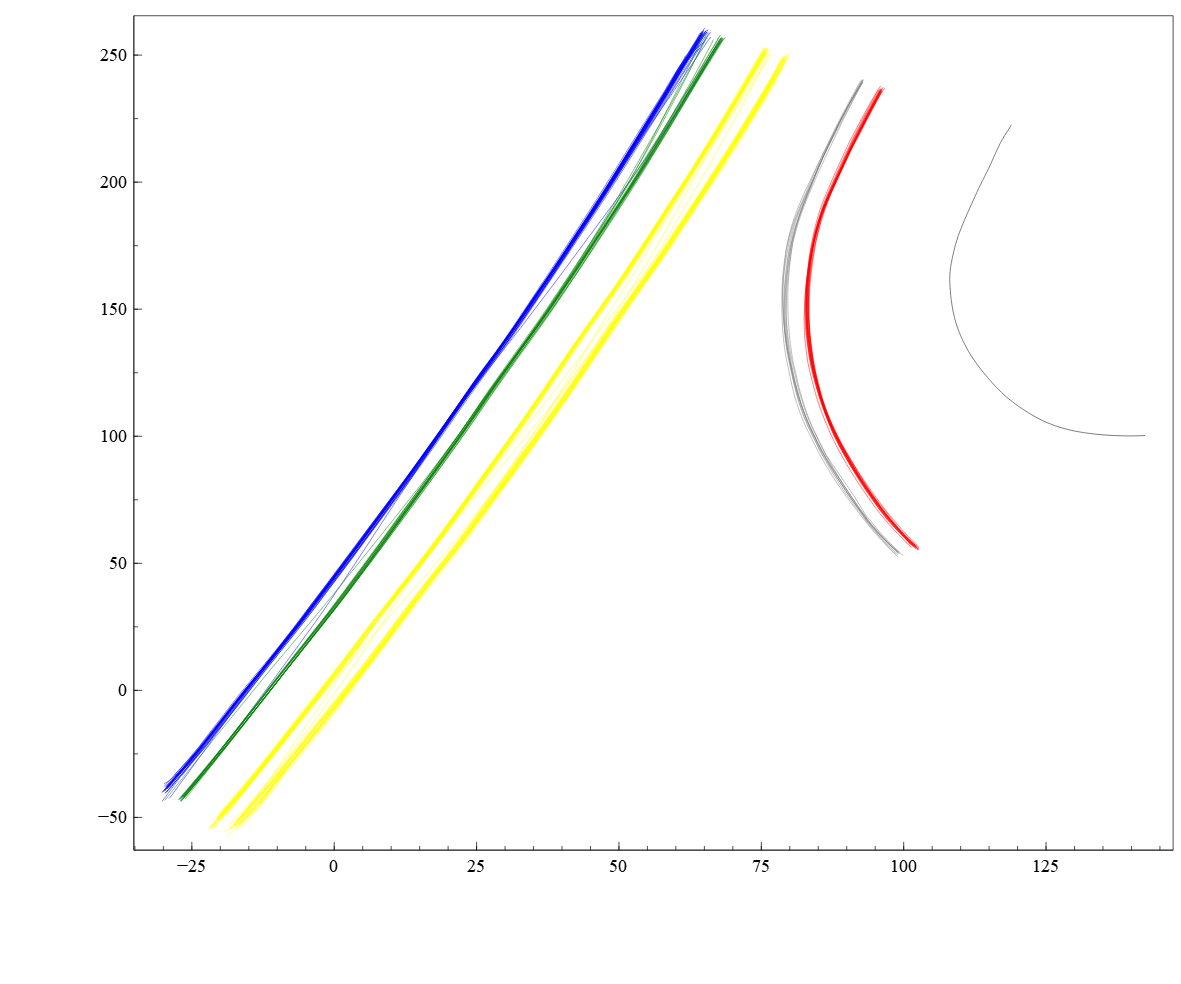
\includegraphics[align=c, width=0.42\linewidth]{../resources/img/umsetzung/U1/atev_results/entennest_k_est}
    }}
    \qquad
    \subfloat[mit fester Clusteranzahl]{{
        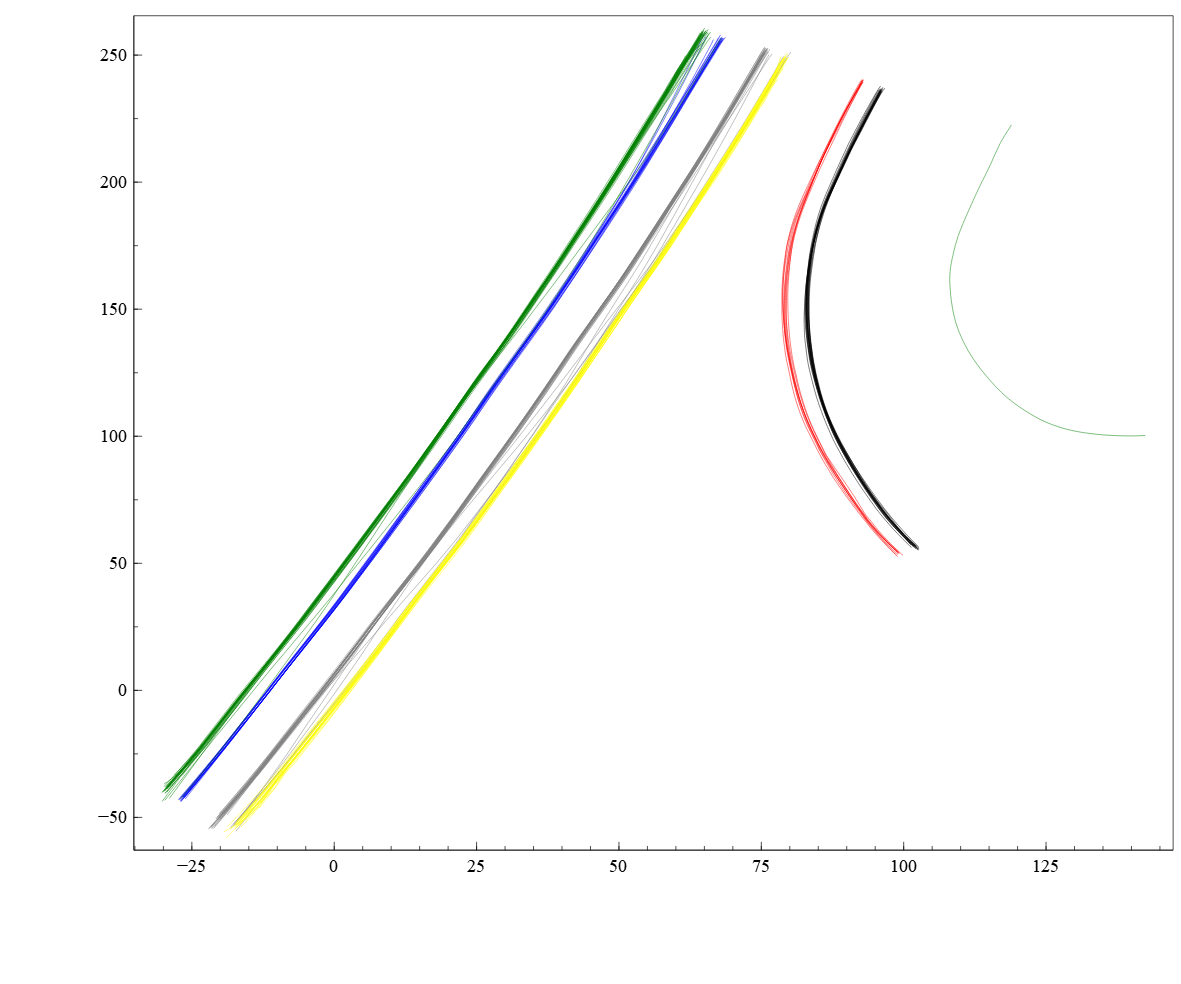
\includegraphics[align=c, width=0.42\linewidth]{../resources/img/umsetzung/U1/atev_results/entennest_k6}
    }}
    \caption{Ergebnisse Clusteranalyse Autobahn (Ansatz Atev et al.)}
    \label{fig:real_results_atev1}
\end{figure}

Die ersten Untersuchungen und Tests des Ansatzes zeigten sehr schnell Schwächen und Grenzen des Vorgehens auf.
Eine Problem sind zum einen die vielen Parameter und Grenzwerte des Verfahrens, welche nicht alle intuitiv
verständlich sind und vom Anwender bestimmt werden müssen. Neben den oben aufgeführten Parametern, gibt es
noch weitere, welche bei der Bestimmung der Clusteranzahl zum Einsatz kommen. Die Parameter wurden
zuerst mit geschätzten, sinnvollen Werten initialisiert und anschließend über verschiedene Tests hinweg optimiert.
Eine weitere Optimierung der Parameter und somit der erzielten Ergebnisse wäre sicherlich möglich gewesen,
hierauf wurde aber aufgrund der weiteren Probleme verzichtet.

Problematisch ist das Vorgehen auch, da der Spectral-Cluster-Algorithmus nicht mit Ausreißern umgehen kann,
welche trotz der Vorverarbeitung der Trajekorien immer noch in den Datensätzen vorhanden seien können.
In Abbildung \ref{fig:real_results_atev1} a) und b) ist beispielsweise die einzelne Fahrspur im oberen, rechten Bereich
einem anderen Spur-Cluster zugeordnet, was nicht korrekt ist.
Diese falsche Zuordnung der Ausreißer, würde die Bestimmung der Spur-Geometrien im nächsten Schritt des
Algorithmus aus \ref{fig:concept_laneDetection_activity} erheblich erschweren.

Die schlechten Clustering-Ergebnisse des Ansatzes sind zudem Folge der nicht zuverlässig funktionierenden Schätzung
der Clusteranzahl $k$. Im Fall des Datensatzes aus Abbildung \ref{fig:real_results_atev1}, wird $k = 5$
statt korrekterweise $k = 6$ geschätzt. Hieraus ergibt sich, dass in a) zwischen zwei Fahrspuren nicht richtig unterschieden wird.
In b) wurde die Clusteranzahl händisch spezifiziert, was in einer korrekten Gruppierung der Fahrspuren resultierte.

Ausschlaggenend dafür, dass der Ansatz von Atev et al. nicht weiter verfolgt und optimiert wurde, war schlussendlich
jedoch die Performance der Clusteranalyse. Für den Trajektorie-Datensatz aus Abbildung \ref{fig:real_results_atev1},
welcher nach der Vorverarbeitung nur 132 Bewegungsbahnen beinhaltet, benötigt die Clusteranalyse bereits über
90 Sekunden. Für einen Datensatz mit über 400 Trajektorien, betrug die Verarbeitungsdauer über 8 Minuten.
Die schlechte Performance lässt sich primär auf das aufwendige Distanzmaß, aber auch auf die mehrfache
Durchführung des k-Means Algorithmus zurückführen.

Aufgrund der oben angeführten Problematiken wurde früh entschieden, dass der Ansatz von Atev et al. nicht weiter
verfolgt werden soll. Es wurde ein Ansatz gesucht, welcher mit den nun entdeckten Herausforderungen besser
umgehen kann.

\subsection{Ansatz DBSCAN und LCSS}
% Ansatz B:
%   LCSS Distanz (in anderen Papern gute Ergebnisse) (impl. mittels bottom up dyna. programmierung, Verwendung Eucl. Dist.)
%   Wieso D2 aus Vlachos et al. verwendet? (Verschiebung unerwünscht)
%   DBSCAN Clustering
%   --> DM kann besser mit Ausreißern umgehen und DBSCAN berücksichtigt diese auch
%   bessere Ergebnisse

\subsection{Erkennung von Abbiegespuren}